\section{Informazioni generali}

\subsection{Descrizione}
SPID, il Sistema Pubblico di Identità Digitale, è la soluzione che permette di accedere a tutti i servizi online della Pubblica Amministrazione con un'unica Identità Digitale (username e password) utilizzabile da computer, tablet e smartphone.
\subsection{Riferimenti Normativi}
Sono state seguite le REGOLE TECNICHE (articolo 4, comma 2, DPCM 24 ottobre 2014).
\\ Sono state seguite anche le regole del sistema previste da SAML v2 per il profilo “Web
Browser SSO”.
\subsection{Funzionamento in breve}
La richiesta di autenticazione SAML può essere inoltrata 
da un Service Provider all’Identity Provider
usando il binding HTTP Redirect o il binding HTTP POST.
\\ La relativa risposta SAML può invece essere inviata
dall’Identity Provider al Service Provider 
solo tramite il binding HTTP POST.

\section{Interfacce logiche}
Esaminando le interfacce logiche si può capire il funzionamento.
\subsection{Interfacce del Identity Provider}
\begin{itemize}
    \item \textbf{IIDPUserInterface}: permette agli utenti l’interazione via web in fase di challenge di autenticazione.
    \item \textbf{IAuthnRequest}: ricezione di richieste di autenticazione SAML.
    \item \textbf{IMetadataRetrieve}: permette il reperimento dei SAML metadata dell’Identity Provider.
\end{itemize}
\subsection{Interfacce del Service Provider}
\begin{itemize}
    \item \textbf{IAuthnResponse}: ricezione delle risposte di autenticazione SAML.
    \item \textbf{IMetadataRetrieve}: permette il reperimento dei SAML metadata del Service Provider.
    \item \textbf{IDSResponse}: ricezione delle risposte da parte del Discovery Service.
\end{itemize}

\pagebreak
\section{Schema Funzionamento}
\subsection{Scenario di Interazione in Modalità SSO}
Di seguito è rappresentato il passaggio di autentificazione nel momento in cui si preme sul pulsante SSO e si viene reindirizzati al Service Provider.
\begin{center}
	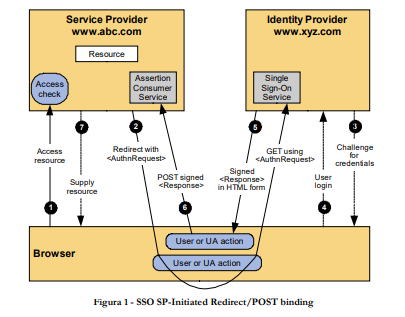
\includegraphics[scale = 1]{./res/images/ScenarioUsoSPIDSchema.PNG}
\end{center}

\section{Scenario Di Utilizzo}
\begin{center}
	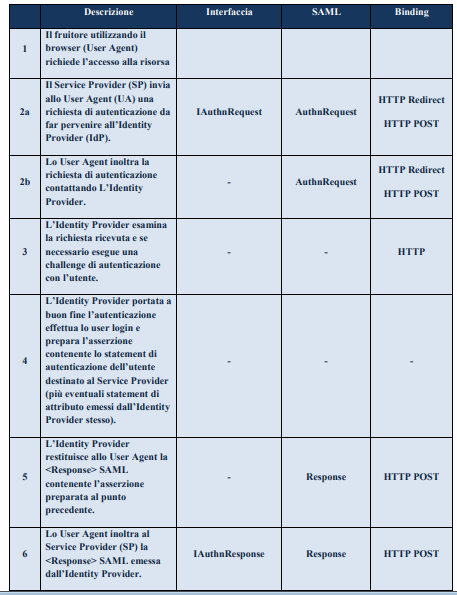
\includegraphics[scale = 1]{./res/images/ScenarioUsoSPID.PNG}
\end{center}

\pagebreak
\section{Binding}
\subsection{Breve descrizione}
Per Binding si intende il momento in cui l'User Agent viene reindirizzato verso un'altro portale durante l'autentificazion;
in particolare dal Service Provider al Identity Provider e in fine per ritornare al primo.
\subsection{BINDING HTTP Redirect}
Service Provider invia allo User Agent un messaggio HTTP di redirezione, cioè avente uno status code con
valore 302 (“Found”) o 303 (“See Other”);
\\ Il Location Header del messaggio HTTP contiene l’URI di destinazione del servizio di Single
Sign-On esposto dall’ Identity Provider.
\\ Il Pacchetto HTTP trasporta i parametri tutti URL-encoded codificato in formato
Base64 e compresso con algoritmo DEFLATE.
\\ Il messaggio all'interno è la risorsa richiesta originaria a cui 
trasferire il controllo una volta terminata l'autenticazione, 
algoritmo e firma per la codifica delle informazioni.
\\ Una volta avute queste informazioni il User Agent fa una 
richiesta GET al Identity Provider con tutte le informazioni 
sopracitate sotto forma di URLENCODED.

\subsection{BINDING HTTP POST}
Service Provider invia allo User Agent un messaggio HTTP con
status code avente valore 200 (“OK”).
\\ Il messaggio HTTP contiene una form HTML codificato come valore di un hidden form
Utilizzando questa metodologia questo permette
di superare i limiti di dimensione della query string.
\\ L’intero messaggio SAML in
formato XML può essere firmato ( XML Digital Signature) 
\\ Il risultato codificato in formato Base64;
\\ Il messaggio all'interno e' la risorsa originaria richiesta 
a cui trasferire il controllo a termine della autentificazione,
Form autopostante attraverso uno script javascript. 
\\ In fine Il browser dell’utente 
elabora quindi la risposta HTTP e invia una richiesta HTTP POST
verso il componente Single Sign-On dell’Identity Provider.

\section{Invio Del Responso}
\subsection{Breve descrizione}
Per Response si intende la risposta che l'Identiry Provider invia al Service Provider con 
l'esito della autentificazione e con le informazioni richieste dal Service Provider appartenente al Utente.
\subsection{Response}
Conclusa la fase di autenticazione, l’Identity Provider costruisce una Response firmata diretta
al Service Provider.
\\ La Response viene inserita in una form HTML come campo nascosto di nome
“SAMLResponse”. 
\\ L’Identity Provider invia la form HTML al browser dell’utente in una risposta
HTTP.
\\ Il browser dell’utente elabora quindi la risposta HTTP e invia una richiesta HTTP POST
contenente la Response firmata verso il Service Provider.

\section{Sicurezza}
\subsection{Accorgimenti Attuati}
Per quanto riguarda la gestione della sicurezza nel canale di trasmissione
si utilizza SSLv.3.0 o TLS 1.0


\section{Metadata}
\subsection{Scopo}
Ogni entità fornisce dei Metadata per dichiarare con trasparenza le proprie carateristiche e i servizi ed informazioni offerte o richieste.
\subsection{Identity Provider METADATA}
metadata conformi allo standard SAMLv2.0.
\begin{itemize}
    \item \textbf{entityID}: indicante l’identificativo (URI) dell’entità univoco in ambito SPID.
    \item \textbf{Protocollo}: Identificatore dei protocolli supportati dalla entità.
    \item \textbf{SingleSignOnService}: Location url endpoint del servizio per la ricezione delle richieste ed il tipo di binding da fare con il service Provider (HTTP-Redirect" oppure HTTP-POST)
    \item \textbf{Organizzazione}: Organizzazione a cui afferisce il identity Provider.
    \item \textbf{Signature}: Segnatura propietaria.
    \item \textbf{Attributi}: Uno o più elementi <attribute> ad indicare nome e formato degli attributi certificabili dell’Identity provider.
    Molto Importante in quanto un sistema simile potremmo utilizzare anche noi.
\end{itemize}
I metadata Identity Provider saranno disponibili per tutte le entità SPID federate attraverso
l’interfaccia IMetadataRetrive alla URL dominioGestoreIdentita/metadata

\subsection{Service Provider METADATA}

\begin{itemize}
    \item \textbf{IMetadataRetrieve}: permette il reperimento dei SAML metadata del Service Provider da parte dell’Identity Provider.
    \item \textbf{IdentityID}: ID indicante l’identificativo univoco (un URI) dell’entità.
    \item \textbf{Chiave}: Chiave pubblica della entità per Signature.
    \item \textbf{Signature}: Segnatura propietaria.
    \item \textbf{AssertionConsumerService}: Il come contattare il service provider con il response, specificando il tipo di binding e il location URI.
    \item \textbf{Organizzazione}: Organizzazione a cui afferisce il Service Provider.
    \item \textbf{Attributi}: Lista attributi che il Service Provider richiede che gli vengano rilasciati dal identity provider (nome, cognome, data nascita, residenza, etc...), Possono essere diversi in base al service name desiderato, i quali possono essere molteplici.
\end{itemize}

\section{Attribute Authority}
\subsection{Descrizione}
Durante il processo di ricerca per il suddetto sistema SPID non si è evidenziato con dettaglio le funzioni di questo attore, si è però 
visto che ha come ruolo la repsonsabilità di verificare le altre due tipologie di enti.
\\ Esso deve essere in grado di certificare un determinato set di attributi relativi ad un soggetto titolare di
una identità digitale. 
\\ A fronte di una richiesta di uno o più attributi l’Attribute Authority deve essere
in grado di:
\begin{itemize}
    \item \textbf{1}. ricevere ed interpretare la richiesta di attributo pervenuta da una Service Provider;
    \item \textbf{2}. elaborare la richiesta;
    \item \textbf{3}. costruire la risposta inerente la richiesta pervenuta ed inoltrarla alla Service Provider.
\end{itemize}

\subsection{Interfacce}
Il componente Attribute Authority deve esporre le seguenti interfacce:
\begin{itemize}
    \item \textbf{IAttributeQuery}: interfaccia applicativa che supporta le operazioni di richiesta di attributo SAML;
    \item \textbf{IMetadataRetrive}: permette il reperimento dei SAML metadata da parte delle Service Provider;
\end{itemize}

\section{Tracciatura Attività}
Le tracciature devono essere mantenute nel rispetto del codice della privacy sotto la responsabilità
titolare del trattamento dell’Identity Provider e l’accesso ai dati di tracciatura deve essere riservato
a personale incaricato.
\\ Si utilizza un (DBMS) in cui viene tenuto traccia per 24 mesi del
a coppia dalla <AuthnRequest> e della relativa < Response>.

\section{Design e Grafica}
Per gestire l’accesso ai servizi pubblici e privati che utilizzano 
il sistema SPID, si rende necessario, sia per una questione di 
user experience che di immagine del sistema, 
la standardizzazione delle interfacce, della comunicazione 
e dell’utilizzo del logo SPID.

\section{Spid Button}
Lo SPID Button consente all'utente la scelta del proprio Identity Provider per l'autenticazione.
Con l'utilizzo di spid-smart-button si intende:
\begin{itemize}
    \item facilitare l'integrazione del bottone "Entra con SPID";
    \item fornire un bottone ospitato via CDN (implementabile tramite javascript e CDN);
    \item migliorare l'esperienza utente.
\end{itemize}

//Codice HTML
<script type="text/javascript" src="https://XXXXXXXXXXXX/spid-button.min.js"></script>
<div id="spid-button">
    <noscript>
        Il login tramite SPID richiede che JavaScript sia abilitato nel browser.
    </noscript>
</div>
//Da inizializzare con una chiamata JavaScript
//Codice Javascript
SPID.init({...});

\section{Linguaggi Di Programmazione e Framework}
Per quanto riguarda lo SPID sono state fornite diverse librerie quasi
per ogni framework, è indifferente la piattaforma infatti esiste una libreria
che permette la sua implementazione ovunque.
\\ Il più semplice e di utilità e' sembrato quello in PHP.
Di seguito ho trovato una demo proprio di questa sua implementazione

\section{Demo Example}
Di seguito è presente il riferimento a una Demo in cui
sono contenuti due Container utilizzabili con Docker, uno per il service provider
ed uno per il identity provider.
\\ \url{https://github.com/simevo/spid-php-lib-example}
\\ Sfortunamente Questa Demo pare obsoleta e non completamente compatibile con tutte le archttetture.


\section{Riferimenti}
Lista delle repo ufficiali per lo SPID:
\\ \url{https://github.com/italia}
\\ Regole Tecniche (articolo 4, comma 2, DPCM 24 ottobre 2014):
\\ \url{https://github.com/italia/spid-regole-tecniche}
\\ \url{https://www.agid.gov.it/sites/default/files/repository_files/circolari/spid-regole_tecniche_v1.pdf}
\\ Riferimenti allo standard grafici e layout:
\\ \url{https://github.com/italia/spid-graphics}
\\ Esempio di Service provider e identity provider Con Docker:
\\ \url{https://github.com/simevo/spid-php-lib-example}
\\ Smart button Spid per autenticazione, in progress ma attualmente da seguire come riferimento:
\\ \url{https://github.com/italia/spid-smart-button}



